% ---------------------------- comment out when compiling the full document -------------------
\documentclass[11pt]{mytustyle}  % default square logo 
\usepackage{amssymb}
\usepackage{caption}
\usepackage{upgreek}
\usepackage[greek,english]{babel}
\usepackage{subfig}
\usepackage{enumitem}
\setlist[description]{leftmargin=0cm,labelindent=0cm}
\begin{document}
\baselineskip=15pt
\newcommand{\ga}{\greektext a\latintext}
\newcommand{\gmu}{\greektext m\latintext}
% ---------------------------------------------------------------------------------------------------------------

\chapter{Signal formation in diamond}
A sensor converts the energy deposited by a particle or a photon and to an electrical signal. There are many types of sensors existing, but in this chapter we will focus on semiconductors, in particular on diamond sensors. Diamond is a good insulator, but behaves as a semiconductor in certain cases. Section~\ref{sec:princsigfor} explains in detail the energy deposition and signal formation mechanism whereas the section~\ref{sec:elecsigproc} focuses on signal amplification and acquisition. Noise contributions are discussed at every stage of the signal chain.


Table~\ref{tab:semicompare} compares the properties of diamond and silicon. 

\begin{footnotesize}
\begin{center}
\captionof{table}{Comparison diamond -- silicon}
\begin{tabular}{   l  c  c   }
\hline
Property & Diamond & Silicon \\
\hline
Band gap energy E$_g$ (eV) & 5.5 & 1.12  \\
Electron mobility $\upmu_e$ (cm$^2$ V$^{-1}$ s$^{-1}$) & 1800 & 1350 \\
Hole mobility $\upmu_h$ (cm$^2$ V$^{-1}$ s$^{-1}$) & 1200 & 450 \\
Breakdown field (V cm$^{-1}$) & $10^{7}$ & $3\times 10^5$ \\
Resistivity ($\Upomega$ cm) & $>10^{11}$  & $2.3\times 10^5$  \\
Intrinsic carrier density (cm$^{-1}$) & $<10^3$ & $1.5\times 10^{10} $ \\
Mass density (g cm$^{-1}$) & $ 3.52$ & $2.33 $ \\
Atomic charge  & $6 $ & $ 14$ \\
Dielectric constant $\upvarepsilon$ & $5.7 $ & $11.9 $ \\
Displacement energy (eV/atom) & $43 $ & $13-20 $ \\
Energy to create an e-h pair  (eV) & $13 $ & $ 3.6$ \\
Radiation length (cm) & $ 12.2$ & $9.6 $ \\
Avg. signal created/$\upmu$m (e) & 36 & 89 \\\hline
\end{tabular}
\label{tab:semicompare}
\end{center}
\end{footnotesize}


% ---------------------------------------------------------------------------------------------------------------
\clearpage
\section{Principles of signal formation in semiconductors}
% ---------------------------------------------------------------------------------------------------------------
\label{sec:princsigfor}
Lattice, electron-hole pair production (3 pg)
Ramo theorem (2 pg)
SC detector systems, pg. 43-73

Semiconductors are materials that are that are conductive only under specific conditions.  They can be made up of atoms with four electrons in their valence band (e.g. silicon--Si, carbon--C or germanium--Ge) or as combinations of two or more different materials (e.g. gallium arsenide--GaAs). 

The atoms form valence bonds with adjacent atoms, making solid crystal structures. These bonds break if sufficient external energy is applied. The electron that was forming the bond is kicked out, leaving behind a positively charged ion with a vacancy in its valence band (see figure~\ref{fig:semilattice9}). A free electron-hole pair is thus created. The free electron travels through the crystal until it is caught by another hole. Similarly, the hole also "travels" through the material. Its positive charge attracts a bound electron in the vicinity, which breaks from the current bond and moves to the vacancy, leaving a new hole behind. The process continues, making it look like the vacancy -- hole is traveling through the material.

\begin{figure}[!t]
\begin{center}
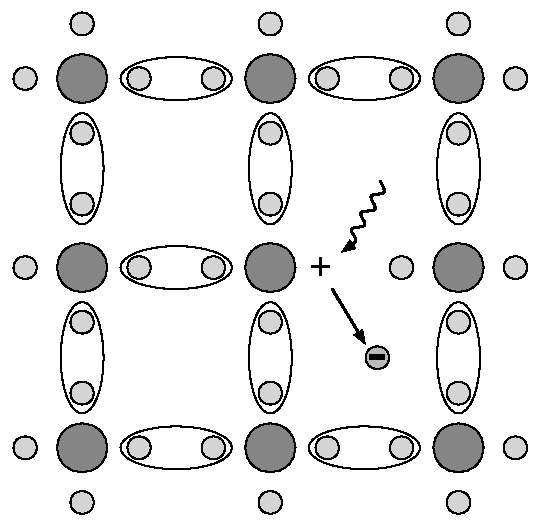
\includegraphics[width=0.4\linewidth]{plots/semilattice9}
\caption{Valence bonds in the crystalline structure can be broken, producing a free electron-hole pair}
\label{fig:semilattice9}
\end{center}
\end{figure}

If an external electric field is applied to the crystalline structure, the free electrons and holes drift toward the positive and negative potential, respectively (see figure~\ref{fig:simpledrift}). While drifting, the charges couple with the electrodes, inducing current in the circuit. They recombine upon reaching the electrodes.


\begin{figure}[!t]
%\centering
\begin{tabular}{cccc}
\subfloat[An electron-hole pair drifting in electric field]{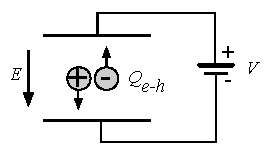
\includegraphics[width=0.45\textwidth]{plots/simpledrift} \label{fig:simpledrift}} &
\subfloat[Equivalent circuit]{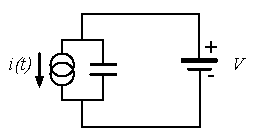
\includegraphics[width=0.45\textwidth]{plots/simpledrifteq}  \label{fig:simpledrifteq}}
\end{tabular}
\caption{Electron-hole drift representation in a circuit}
\end{figure}

The electrons need to absorb a certain energy to get kicked out of the atomic bond -- ionised. The minimal energy required to excite (ionise) an electron in a semiconductor is equal to the energy gap $E_g$. Typical widths of the forbidden gap are 0.7~eV in Ge, 1.12~eV in Si, 1.4~eV in GaAs and 5.5~eV in Di.

Due to the small band gap in semiconductors some electrons occupy the conduction band at room temperature (RT). The intrinsic carrier concentration $n_i$ in semiconductors is given as
\begin{equation}
\label{eq:intrinsiccarrier}
n_i = T^{3/2} \cdot exp(-\frac{E_g}{2kT}) 
\end{equation} 
wherein $k = 1.381\cdot10{-23}m^2 kg s{-2} K{-1}$ is the Boltzmann constant and T is the temperature.


XXXXXXXXX




\begin{figure}[!t]
\begin{center}
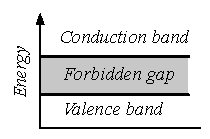
\includegraphics[width=0.4\linewidth]{plots/energygap}
\caption{Energy states of an electron}
\label{fig:energygap}
\end{center}
\end{figure}




\subsubsection{Thermal noise in semiconductors}







\subsection{Signal charge fluctuations}
%The amplitude of the signal is subject to statistical fluctuations.
Two of the important sensor characteristics are the magnitude of the signal and the fluctuations of the signal at a given absorbed energy. They determine the relative resolution $\Updelta$E/E. For semiconductors the signal fluctuations are smaller than the simple statistical variance $\upsigma_Q=\sqrt{N_Q}$, where N$_Q$ is the number of released charge pairs (ratio between the total deposited energy E$_0$ and the average emergy deposition E$_i$ required to produce a charge pair). In fact, \cite{} shows that the variance is $\upsigma_Q=\sqrt{F N_Q}$, where F is the Fano factor~\cite{} (0.08 for diamond and 0.115 for silicon ~\cite{}). Thus, the variance of the signal charge is smaller than expected, $\upsigma_Q\approx0.3 \sqrt{N_Q}$. The resulting intrinsic resolution of semiconductor detectors is 
\begin{equation}
\label{eq:efwhm}
\Updelta E_{FWHM} = 2.35 \sqrt{FEE_i} 
\end{equation} 
wherein Si E$_i$= 3.6~eV and C E$_i$= 13~eV. E.g., for an \ga particle with energy E$_\alpha$ = 5.486 MeV the calculated $\Updelta$E$_{\alpha FWHM}$ = 5.6~keV. Figure~\ref{fig:enerres} shows the energy resolution function for silicon and diamond.


\begin{figure}[!t]
\begin{center}
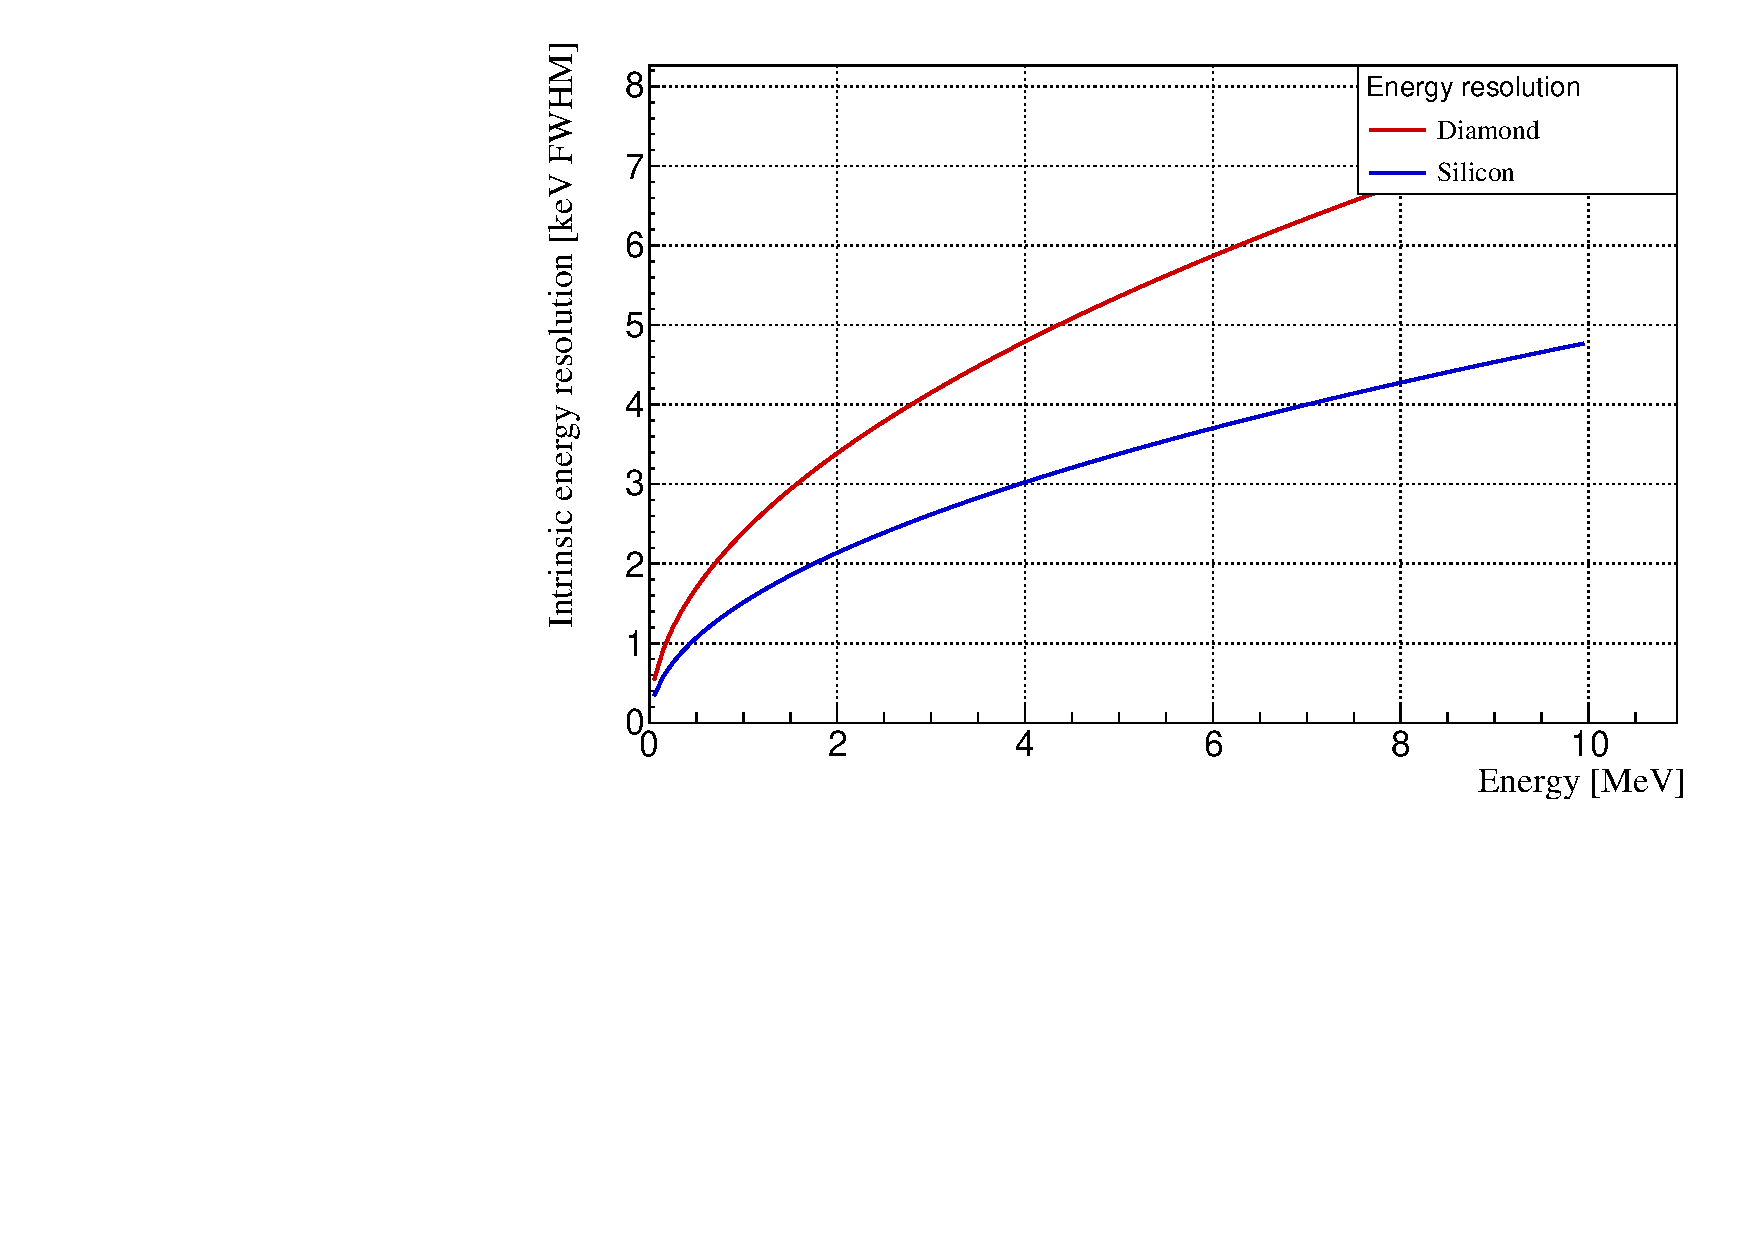
\includegraphics[width=0.8\linewidth]{plots/Intrinsic_energy_res}
\caption{Intrinsic energy resolution for silicon and diamond}
\label{fig:enerres}
\end{center}
\end{figure}


%The energy from an incoming particle can be absorbed by lattice excitation (phonon production) or by ionisation (formation of a mobile charge pair). For a single event, the deposited energy E$_{0}$ is equal to the sum of the energies going into excitation (E$_{ex}$) and ionisation (E$_{ion}$)
%\begin{equation}
%\label{eq:excitationionisation}
%E_0 = E_{ex} N_{ex} + E_{ion} N_{ion}
%\end{equation} 
%where N$_{ex}$ is the number of excitations (phonos produced) and N$_Q$ is the number of charge pairs released. For this event, if more 






\subsection{Signal formation}


\subsection{Radiation-induced electrical pulses}

Theory: Examples - average pulses - persistence - gamma, beta, alpha		

Current profiles
Alpha
beta
gamma
neutron


% ---------------------------------------------------------------------------------------------------------------
\clearpage
\section{Carrier transport in a diamond sensor} % signal acquisition
% ---------------------------------------------------------------------------------------------------------------
This section describes the carrier transport phenomena in diamond. This theory provides the basis for discussion about the measurements in chapter~\ref{XXXCHAPTER}. 

Free charge carriers in a semiconductor get thermally excited and scatter in random directions with a thermal velocity $v_{th}$. Their integral movement due to thermal excitation equals zero. Their transport is instead by means of drift and diffusion. Diffusion is caused by the concentration gradient. In its presence the carriers tend to scatter in the direction of the lower concentration. Drift on the other hand is caused by an externally applied electrical field. In that case the carriers move in parallel to to the field lines. In a sensor with a high applied field the diffusion contribution is negligible. 

\begin{description}

\item[Diffusion]
The concentration profile dissolves with time forming a Gaussian distribution with variance $\sigma(t)=\sqrt{Dt}$. 

\item[Drift velocity and mobility]
The charge carriers drift through the diamond bulk with a drift velocity $v_{drift}(E)$, which is proportional to the electric field $E$ at low electric fields: $v_{drift} = \mu E$. The proportionality factor $\mu$ is defined as the mobility in cm$^2$V$^{-1}$s$^{-1}$. For higher fields, however, the velocity saturates. The final equation for $v_{drift}$ is therefore
\begin{equation}
\label{eq:vsat}
v_{drift}(E) = \mu(E)E= \frac{\mu_0 E}{1 + \frac{\mu_o E}{v_{sat}}}
\end{equation}

where $\mu_0$ is the low drift mobility and $v_{sat}$ is saturation velocity. The drift velocity can be retrieved experimentally via the transit time measured with so-called Transient Current Technique (TCT). This technique enables the measurement of transit time $t_t$ of the carriers through the sensor with the thickness $d$. 

\begin{equation}
\label{eq:vsat}
v_{drift}(E) = \frac{d}{t_t(E)}.
\end{equation}

The velocities for holes and electrons usually differ. 

\item[Velocity saturation]
At higher velocities the carriers lose more energy to the lattice (phonon transport).

\item[Space carge]


\end{description}













% ---------------------------------------------------------------------------------------------------------------
\clearpage
\section{Electronics for signal processing} % signal acquisition
% ---------------------------------------------------------------------------------------------------------------
\label{sec:elecsigproc}
This section describes the electronics of a detector, starting with description of signal amplifiers and then discussing the digitisation and signal processing.

\subsection{Signal preamplifiers}
(2 pg)
The signal charge generated in the sensor is of the order of fC and has to be pre-amplified before processing. The preamplifiers have to be designed carefully to minimise electronic noise while maximising gain -- thus maximising signal-to-noise ratio (SNR). A critical parameter is the total capacitance, i.e. sensor capacitance and input capacitance of the preamplifier. Decreased capacitance improves the SNR. 

Several types of amplifiers can be used, all of which affect the measured pulse shape. They behave differently for resistive or capacitive sources. Given that semiconductors are capacitive sources, we will focus on these. Two preamplifiers are used most commonly, a current and a charge amplifier. Both are described below in detail. 


\subsubsection{Current-sensitive amplifier}
(0.5 pg)
Figure~\ref{fig:curramp} shows the equivalent circuit of a capacitive source and a current amplifier. An amplifier operates in current mode if the source has a low charge collection time $t_c$ with respect to the $RC$ time constant of the circuit. In this case the sensor capacitance discharges rapidly and the output voltage is proportional to the instantaneous current $v_o \propto i_s(t)$. The amplifier is providing voltage gain, so the output signal voltage $v_o$ is directly proportional to the input voltage $v_i$.

\begin{figure}[!t]
\begin{center}
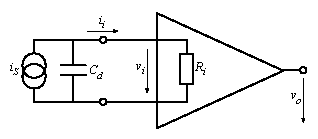
\includegraphics[width=0.6\linewidth]{plots/curramp}
\caption{Simplified equivalent circuit of a capacitive source and a current amplifier}
\label{fig:curramp}
\end{center}
\end{figure}


\subsubsection{Charge-sensitive amplifier}
(0.5 pg)
In order to measure integrated charge in the sensor, a feedback loop is added to the amplifier (see figure~\ref{fig:chgamp}). The feedback can be used to control the gain and input resistance, as well as integrating the input signal. The charge amplifier is in principle an inverting voltage amplifier with a high input resistance. 
 
In an ideal amplifier the output voltage $v_o$ equals $-Av_i$. Therefore voltage difference across the capacitor $C_f$ is $V_f=(A+1)v_i$ and the charge deposited on the capacitor $Q_f=C_f v_f = C_f (A+1)v_i$. Since no current can flow into the amplifier, all of the signal current must charge up the feedback capacitance, so $Q_f = Q_i$.

In reality, however, charge-sensitive amplifiers respond much slower to the than the time duration of the current pulse from the sensor. 


\begin{figure}[!t]
\begin{center}
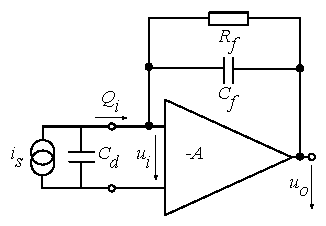
\includegraphics[width=0.6\linewidth]{plots/chgamp}
\caption{Simplified equivalent circuit of a capacitive source and a charge amplifier}
\label{fig:chgamp}
\end{center}
\end{figure}

\subsubsection{Analogue electronic noise}
(2 pg)
Electronic noise determines the ability of a system to distinguish signal levels.

\subsection{Analogue-to-digital converters}
(1 pg)
An analog-to-digital converter (ADC) is a device that converts analogue electrical signal on the input to its digital representation - a digital number. This involves a quantisation -- \emph{sampling} of the signal at a defined sampling period, resulting in a sequence of samples at a discrete time and a discrete amplitude. The resolution of the ADC is the number of output levels it can quantise to and is expressed in bits. For instance, an 8-bit ADC with an input voltage range of 100~mV and a sampling period of 1~ns would produce 1~GSPS (gigasample per second) at a voltage resolution $Q$ of 
\begin{equation}
\label{eq:mvpercnt}
Q=\frac{Input~voltage~range}{2^{~resolution}}  = \frac{100~mV}{2^8~ADC counts} = 0.39~mV/ADC count
\end{equation} 


\subsubsection{Quantisation error and quantisation noise}
(1 pg)
The quantisation error (or a round-off error) is a contribution of the digitisation to the overall measurement error. It is defined as a difference between the actual analog value and a digitised representation of this value.

Typically, the input signal amplitude is much larger than than the voltage resolution. Therefore the quantisation error is not directly correlated with the signal and has an approximately uniform distribution. 


\subsection{Signal processing}
(1 pg)
After signal amplification and digitisation the data can be either processed immediately or they can be saved to a data storage for later analysis. Below are the examples of systems that carry out the data processing on the fly.

\subsubsection{Field programmable gate array}
(0.5 pg)
Field programmable gate array (FPGA) is an integrated circuit designed to be reprogrammable and configured after manufacturing. It consists of a set of logic gates that can be interconnected in numerous combinations to carry out a logic operation. Many such logic operations can take place in parallel, making the FPGA a powerful tool for signal processing.


\subsubsection{Application-specific integrated circuit}
FE-I4 functional description, characteristics
 (2 pg)

Application-specific integrated circuit (ASIC) is an integrated circuit designed for a specific use. The design cannot be modified after chip production, as opposed to FPGAs. On the other hand, the ASICs can be optimised to perform a required operation at high speed and low power. 

 
\subsection{Full detector readout chain}
(1 pg)


% ---------------------------- comment out when compiling the full document -------------------
\end{document}
% ---------------------------------------------------------------------------------------------------------------